\title{Anexo A. Resultados de Comparación de las Eficiencias de ICB}


Percentil-NVC

\begin{figure}[ht] 
	\centering 
	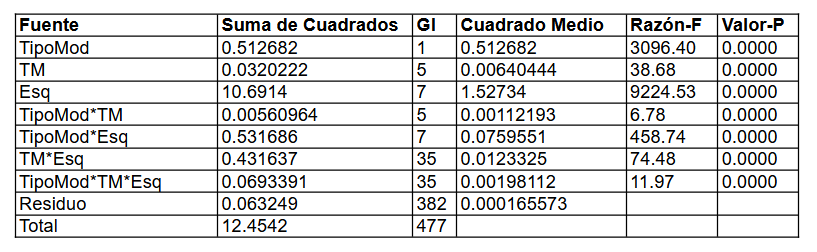
\includegraphics[width=0.95\linewidth]{img/ANOVA_Efic_ICB_Perc_NVC.png} 
	\caption{ANOVA para la eficiencia del ICB Percentil cuando se tiene NVC.} 
	\label{fig:ANOVA_Efic_ICB_Perc_NVC}
\end{figure}
\FloatBarrier


\begin{figure}[ht] 
	\centering 
	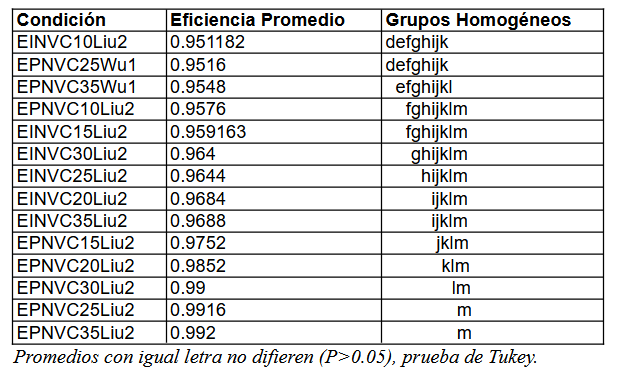
\includegraphics[width=0.76\linewidth]{img/CompEfic_PromICB_Perc_NVC.png} 
	\caption{Comparación de eficiencias promedio del ICB Percentil cuando se tiene NVC.} 
	\label{fig:CompEfic_PromICB_Perc_NVC}
\end{figure}
\FloatBarrier



BCa-NVC

\begin{figure}[ht] 
	\centering 
	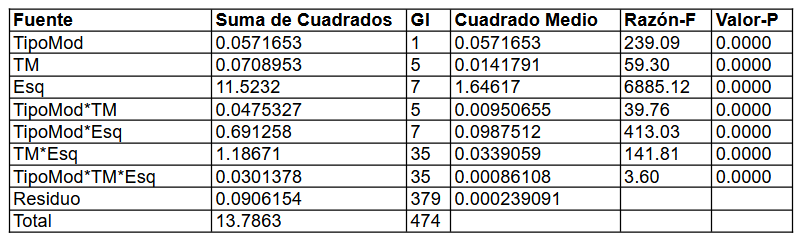
\includegraphics[width=0.95\linewidth]{img/ANOVA_Efic_ICB_BCa_NVC.png} 
	\caption{ANOVA para la eficiencia del ICB BCa cuando se tiene NVC.} 
	\label{fig:ANOVA_Efic_ICB_BCa_NVC}
\end{figure}
\FloatBarrier


\begin{figure}[ht] 
	\centering 
	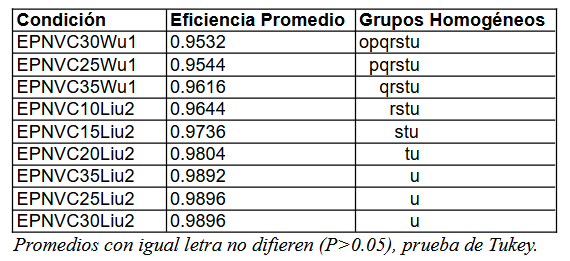
\includegraphics[width=0.76\linewidth]{img/CompEfic_PromICB_BCa_NVC.png} 
	\caption{Comparación de eficiencias promedio del ICB BCa cuando se tiene NVC.} 
	\label{fig:CompEfic_PromICB_BCa_NVC}
\end{figure}
\FloatBarrier



%%%%%%%%%%%%%%%%%%%%%%%%%%%%%%%%%%%%%%%%%%%5

Percentil-NNVC

\begin{figure}[ht] 
	\centering 
	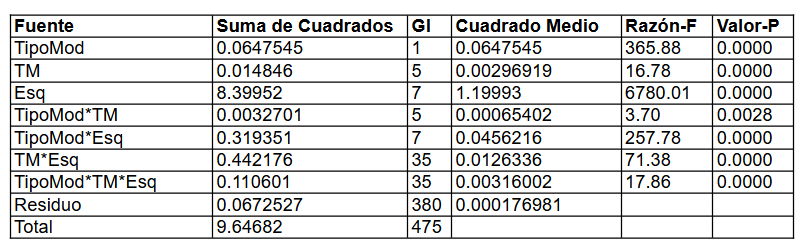
\includegraphics[width=0.95\linewidth]{img/ANOVA_Efic_ICB_Perc_NNVC.png} 
	\caption{ANOVA para la eficiencia del ICB Percentil cuando se tiene NNVC.} 
	\label{fig:ANOVA_Efic_ICB_Perc_NNVC}
\end{figure}
\FloatBarrier


\begin{figure}[ht] 
	\centering 
	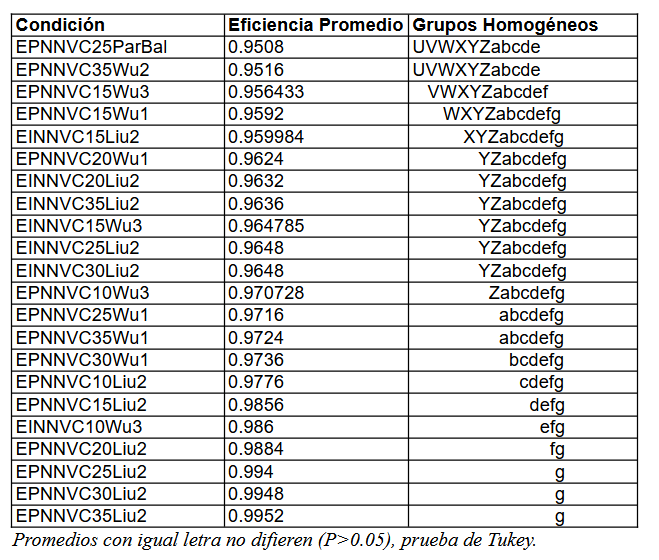
\includegraphics[width=0.76\linewidth]{img/CompEfic_PromICB_Perc_NNVC.png} 
	\caption{Comparación de eficiencias promedio del ICB Percentil cuando se tiene NNVC.} 
	\label{fig:CompEfic_PromICB_Perc_NNVC}
\end{figure}
\FloatBarrier



BCa-NNVC

\begin{figure}[ht] 
	\centering 
	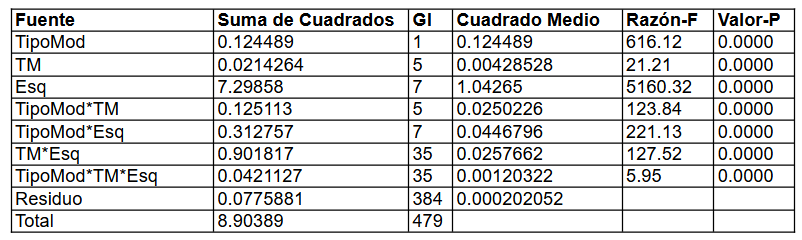
\includegraphics[width=0.95\linewidth]{img/ANOVA_Efic_ICB_BCa_NNVC.png} 
	\caption{ANOVA para la eficiencia del ICB BCa cuando se tiene NNVC.} 
	\label{fig:ANOVA_Efic_ICB_BCa_NNVC}
\end{figure}
\FloatBarrier


\begin{figure}[ht] 
	\centering 
	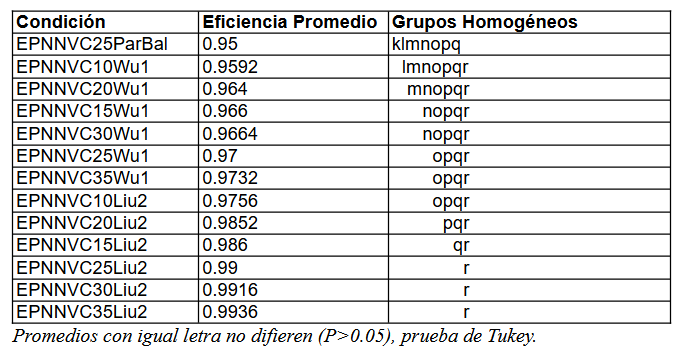
\includegraphics[width=0.76\linewidth]{img/CompEfic_PromICB_BCa_NNVC.png} 
	\caption{Comparación de eficiencias promedio del ICB BCa cuando se tiene NNVC.} 
	\label{fig:CompEfic_PromICB_BCa_NNVC}
\end{figure}
\FloatBarrier



%%%%%%%%%%%%%%%%%%%%%%%%%%%%%%%%%%%%%%%%%%%5

Percentil-NVD

\begin{figure}[ht] 
	\centering 
	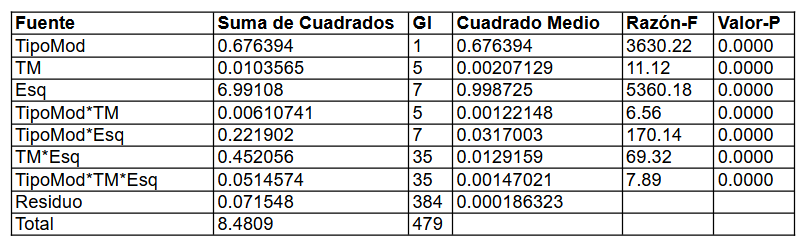
\includegraphics[width=0.95\linewidth]{img/ANOVA_Efic_ICB_Perc_NVD.png} 
	\caption{ANOVA para la eficiencia del ICB Percentil cuando se tiene NVD.} 
	\label{fig:ANOVA_Efic_ICB_Perc_NVD}
\end{figure}
\FloatBarrier


\begin{figure}[ht] 
	\centering 
	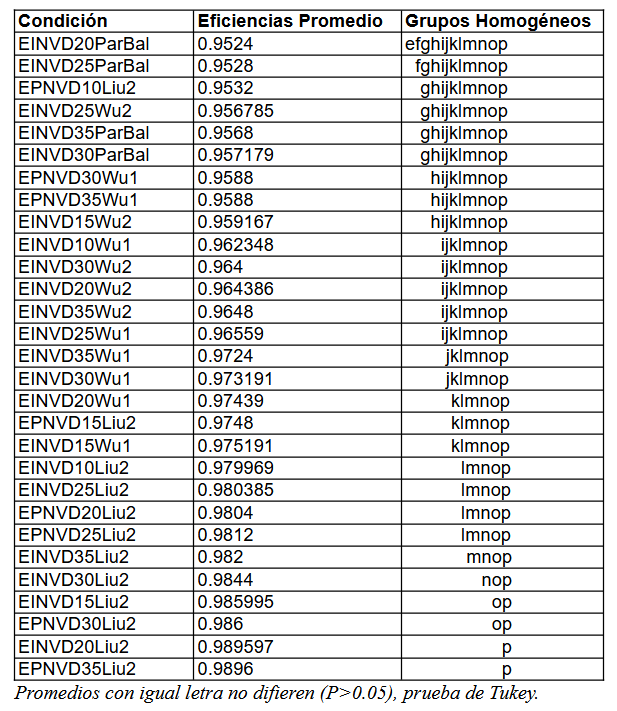
\includegraphics[width=0.76\linewidth]{img/CompEfic_PromICB_Perc_NVD.png} 
	\caption{Comparación de eficiencias promedio del ICB Percentil cuando se tiene NVD.} 
	\label{fig:CompEfic_PromICB_Perc_NVD}
\end{figure}
\FloatBarrier



BCa-NVD

\begin{figure}[ht] 
	\centering 
	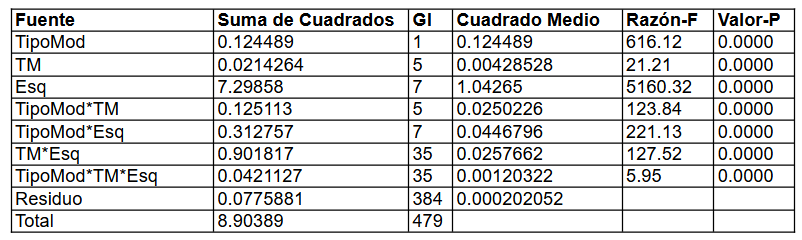
\includegraphics[width=0.95\linewidth]{img/ANOVA_Efic_ICB_BCa_NNVC.png} 
	\caption{ANOVA para la eficiencia del ICB BCa cuando se tiene NNVC.} 
	\label{fig:ANOVA_Efic_ICB_BCa_NNVC}
\end{figure}
\FloatBarrier


\begin{figure}[ht] 
	\centering 
	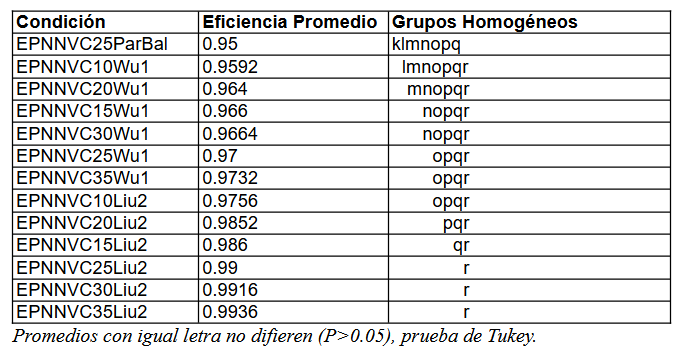
\includegraphics[width=0.76\linewidth]{img/CompEfic_PromICB_BCa_NNVC.png} 
	\caption{Comparación de eficiencias promedio del ICB BCa cuando se tiene NNVC.} 
	\label{fig:CompEfic_PromICB_BCa_NNVC}
\end{figure}
\FloatBarrier





\subsection{Propuesta Final}

Con base en los resultados de los análisis estadísticos, cuando se tenga NVC, NNVC o NVD y se evalué la precisión el ICB a utilizar sería Percentil con esquema de remuestreo Liu2. Y cuando se tenga NNVD y se evalué la precisión, el ICB a utilizar sería BCa con esquema de remuestreo ParBal.


\subsubsection{Implementación}

\subsubsection{Aplicación}

  